% Created 2025-05-24 Sat 11:36
% Intended LaTeX compiler: pdflatex
\documentclass[11pt]{article}
\usepackage[utf8]{inputenc}
\usepackage[T1]{fontenc}
\usepackage{graphicx}
\usepackage{longtable}
\usepackage{wrapfig}
\usepackage{rotating}
\usepackage[normalem]{ulem}
\usepackage{amsmath}
\usepackage{amssymb}
\usepackage{capt-of}
\usepackage{hyperref}
\usepackage[utf8]{inputenc}
\usepackage{graphicx}
\usepackage{hyperref}
\usepackage{listings}
\usepackage{xcolor}
\lstset{basicstyle=\ttfamily\footnotesize,breaklines=true,columns=fullflexible}
\author{YAMASHITA Takao}
\date{\today}
\title{ac1965's Emacs literate configuration \texttt{.emacs.d}}
\hypersetup{
 pdfauthor={YAMASHITA Takao},
 pdftitle={ac1965's Emacs literate configuration \texttt{.emacs.d}},
 pdfkeywords={},
 pdfsubject={},
 pdfcreator={Emacs 31.0.50 (Org mode 9.7.11)},
 pdflang={English}}
\begin{document}

\maketitle
\tableofcontents

\begin{center}
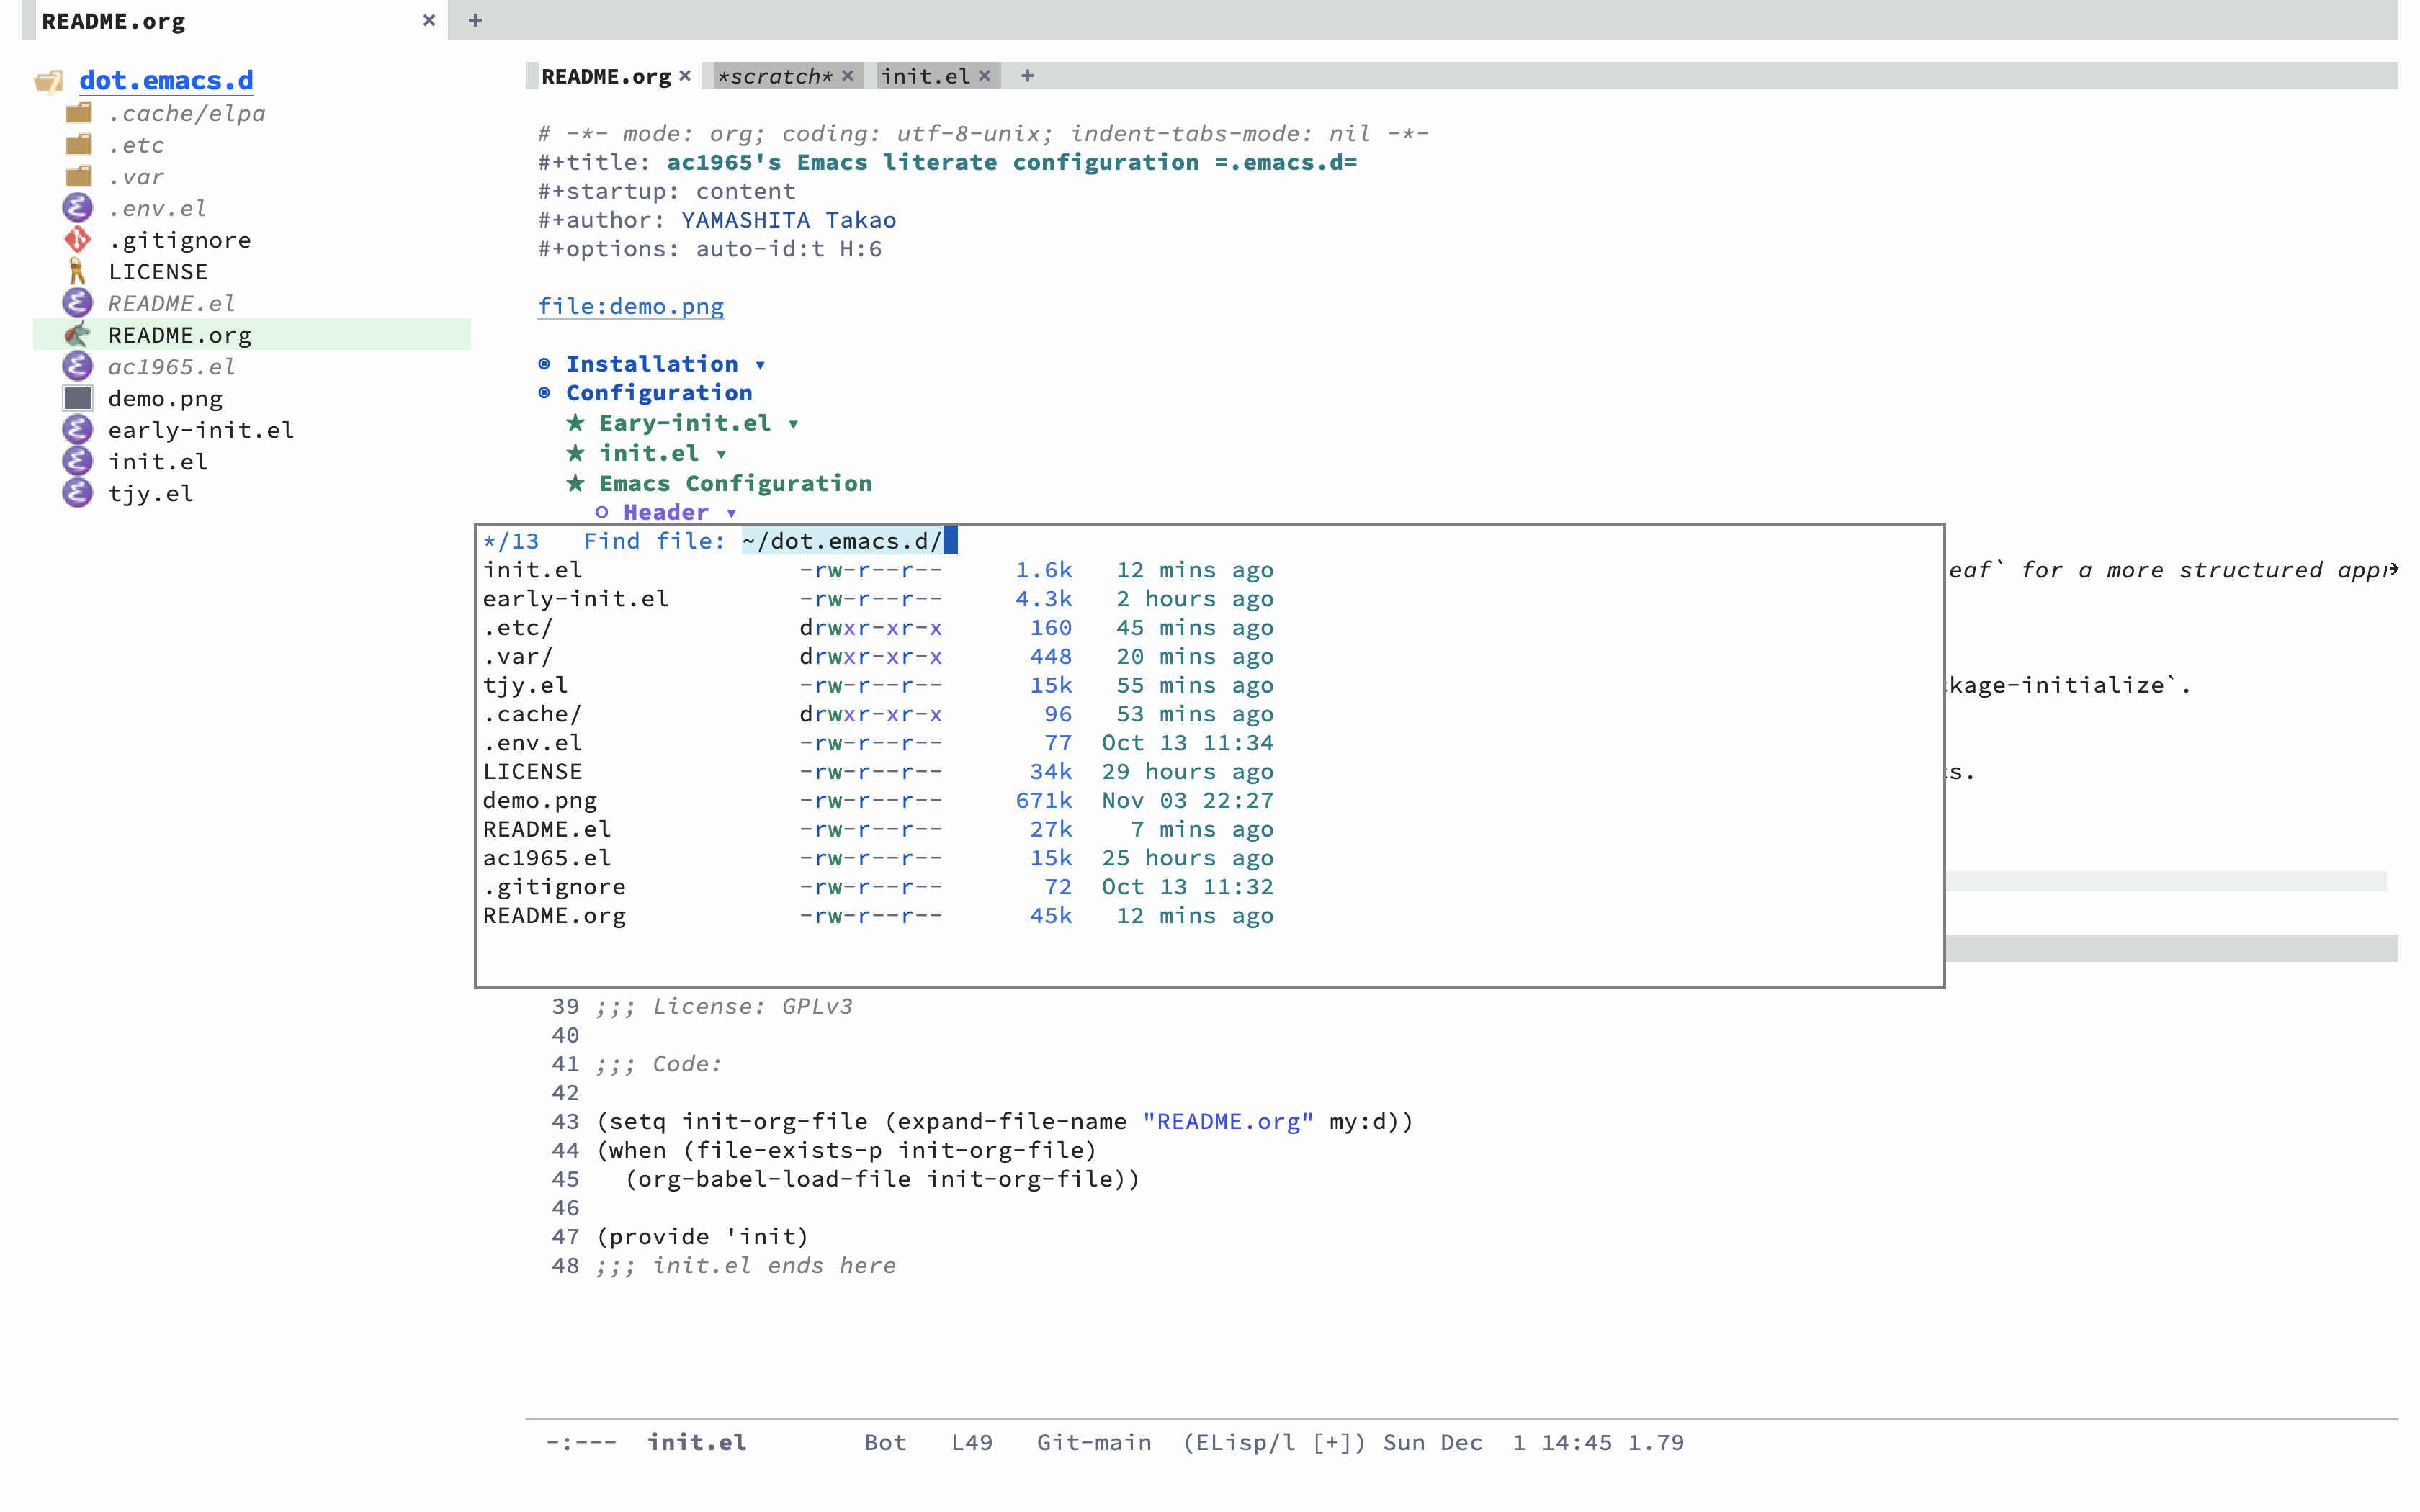
\includegraphics[width=.9\linewidth]{demo.png}
\end{center}
\section{Installation}
\label{sec:org03e3983}

This section documents the steps to build and install Emacs from source safely and effectively.
\subsection{Step 1: Clone the Configuration Repository}
\label{sec:org8435ea8}
Run the following command to clone the configuration files from GitHub:

\begin{verbatim}
git clone --depth 1 https://github.com/ac1965/.emacs.d ~/.emacs.d
\end{verbatim}

Make sure that the \texttt{\textasciitilde{}/.emacs.d} directory does not already exist, or back it up if necessary.
\subsection{Step 2: Build Emacs}
\label{sec:org51f9f73}

To build Emacs, use the provided \texttt{build-emacs.sh} script.
\href{https://github.com/ac1965/dotfiles/blob/master/.local/bin/build-emacs.sh}{ build-emacs.sh}

\begin{verbatim}
build-emacs.sh --native-compilation
\end{verbatim}
\subsection{Requirements and Troubleshooting}
\label{sec:org16de500}

\begin{itemize}
\item \textbf{Dependencies}: Ensure you have the following installed before running the script:
\begin{itemize}
\item `gcc` (Version 10 or newer)
\item `libgccjit`
\item `make`
\end{itemize}

\item \textbf{Permissions}: If you encounter permission issues, try running the script with `sudo`, but only after verifying its contents.

\item \textbf{Error Handling}:
\begin{itemize}
\item If native compilation fails, check that `libgccjit` is installed and properly linked.
\item Verify that the `GITHUB\textsubscript{REPOS}` directory exists and contains the necessary source files.
\end{itemize}
\end{itemize}
\subsection{System Information}
\label{sec:org1863256}

Below are the system details and Emacs build configurations for two machines.

\textbf{New Machine}

\begin{verbatim}
uname -a
Darwin pooh.local 24.4.0 Darwin Kernel Version 24.4.0: Fri Apr 11 18:32:05 PDT 2025; root:xnu-11417.101.15~117/RELEASE_ARM64_T8132 arm64
\end{verbatim}

\begin{itemize}
\item GNU Emacs 31.0.50
\end{itemize}

\begin{center}
\begin{tabular}{ll}
Commit & 0de59ded25aa9f1751edb7170c51a98be70b7edf\\
Branch & master\\
System & aarch64-apple-darwin24.4.0\\
Date & 2025-05-19 23:18:43 (JST)\\
Patch & without ns-inline.patch\\
Features & ACL DBUS GLIB GNUTLS LCMS2 LIBXML2 MODULES NATIVE\textsubscript{COMP} NOTIFY KQUEUE NS PDUMPER PNG RSVG SQLITE3 THREADS TOOLKIT\textsubscript{SCROLL}\textsubscript{BARS} TREE\textsubscript{SITTER} WEBP XIM XWIDGETS ZLIB\\
Options & --with-native-compilation --with-gnutls=ifavailable --with-json --with-modules --with-tree-sitter --with-xml2 --with-xwidgets --with-librsvg --with-mailutils --with-native-image-api --with-cairo --with-mac --with-ns CPPFLAGS=-I/opt/homebrew/opt/llvm/include 'LDFLAGS=-L/opt/homebrew/opt/llvm/lib -L/opt/homebrew/opt/llvm/lib/c++ -Wl,-rpath,/opt/homebrew/opt/llvm/lib/c++'\\
\end{tabular}
\end{center}

\textbf{OLD Machine}

\begin{verbatim}
uname -a
Darwin alice.local 24.3.0 Darwin Kernel Version 24.3.0: Fri Dec  9 19:45:54 PST 2024; root:xnu-11215.80.501.2~1/RELEASE_x86_64 x86_64
\end{verbatim}

\begin{itemize}
\item GNU Emacs 31.0.50
\end{itemize}

\begin{center}
\begin{tabular}{ll}
Commit & aa12cebaa684d7b3ea7e131666d33bcc71b45625\\
Branch & master\\
System & x86\textsubscript{64}-apple-darwin24.4.0\\
Date & 2025-03-23 10:35:38 (JST)\\
Patch & without ns-inline.patch\\
Features & ACL DBUS GIF GLIB GMP GNUTLS JPEG LCMS2 LIBXML2 MODULES NATIVE\textsubscript{COMP} NOTIFY KQUEUE NS PDUMPER PNG RSVG SQLITE3 THREADS TIFF TOOLKIT\textsubscript{SCROLL}\textsubscript{BARS} TREE\textsubscript{SITTER} WEBP XIM XWIDGETS ZLIB\\
Options & --with-native-compilation --with-gnutls=ifavailable --with-json --with-modules --with-tree-sitter --with-xml2 --with-xwidgets --with-librsvg CFLAGS=-I/Library/Developer/CommandLineTools/SDKs/MacOSX.sdk/usr/include CPPFLAGS=-I/usr/local/opt/llvm/include 'LDFLAGS=-L/usr/local/opt/llvm/lib -L/usr/local/opt/llvm/lib/c++ -Wl,-rpath,/usr/local/opt/llvm/lib/c++'\\
\end{tabular}
\end{center}
\section{Emacs Configuration}
\label{sec:org9ec799b}
\subsection{Early Initialization}
\label{sec:orge4ff6a2}

\begin{verbatim}
;;; early-init.el --- My early-init script -*- coding: utf-8 ; lexical-binding: t; -*-

;; Copyright (c) 2021-2025 YAMASHITA Takao <ac1965@ty07.net>
;; Licensed under the GNU General Public License version 3 or later.

;; $Lastupdate: 2025/05/24 11:38:51 $

;;; Commentary:
;; It is designed for Emacs 30 and above, providing essential settings while eliminating redundancy.

;;; Code:

;; ---------------------------------------------------------------------------
;;; Compatibility Check (Emacs 30+)
(when (version< emacs-version "30")
  (error "This configuration requires Emacs 30 or higher."))

;; ---------------------------------------------------------------------------
;;; Directories
(defvar my:d (if load-file-name
                 (file-name-directory (file-chase-links load-file-name))
               user-emacs-directory)
  "Base directory for user-specific configuration.")

(defvar my:d:cache (expand-file-name ".cache/" my:d)
  "Cache directory for temporary files.")
(make-directory my:d:cache t) ;; Ensure cache directory exists

;; ---------------------------------------------------------------------------
;;; Performance Optimization
(setq gc-cons-threshold (* 128 1024 1024)
      read-process-output-max (* 8 1024 1024))

(add-hook 'emacs-startup-hook
          (lambda ()
            (setq gc-cons-threshold (* 64 1024 1024))
            (message "Emacs loaded in %.2f seconds with %d garbage collections."
                     (float-time (time-subtract after-init-time before-init-time))
                     gcs-done)))

(setq package-enable-at-startup nil)

;; ---------------------------------------------------------------------------
;;; Native Compilation Optimization
(setq native-comp-async-report-warnings-errors 'error)
(setq native-comp-async-jobs-number (or (getenv "EMACS_NATIVE_COMP_JOBS") 4))
(setq native-comp-speed 2)
(when (boundp 'native-comp-eln-load-path)
  (startup-redirect-eln-cache
   (expand-file-name "eln-cache/" my:d:cache)))

;; ---------------------------------------------------------------------------
;;; macOS Specific Settings
(when (eq system-type 'darwin)
  ;; Homebrew and GCC Paths
  (dolist (path '("/opt/homebrew/bin" "/usr/local/bin"))
    (when (file-directory-p path)
      (add-to-list 'exec-path path)
      (setenv "PATH" (concat path ":" (getenv "PATH")))))

  ;; GNU ls (gls) for Dired
  (when (executable-find "gls")
    (setq insert-directory-program "gls"
          dired-use-ls-dired t
          dired-listing-switches "-aBhl --group-directories-first")))

;; ---------------------------------------------------------------------------
;;; UI Customization
(setq frame-resize-pixelwise t)
(add-to-list 'default-frame-alist '(fullscreen . maximized))
(menu-bar-mode -1)
(tool-bar-mode -1)
(scroll-bar-mode -1)
(pixel-scroll-precision-mode 1)

;; ---------------------------------------------------------------------------
;;; Miscellaneous Optimizations
(setq inhibit-startup-screen t
      initial-scratch-message nil
      initial-major-mode 'text-mode
      use-short-answers t
      create-lockfiles nil
      display-line-numbers-type 'relative)

\end{verbatim}
\subsection{Main Initialization}
\label{sec:org8fcc6b7}

\begin{verbatim}
;;; init.el --- Main configuration file -*- coding: utf-8 ; lexical-binding: t; -*-

;; Copyright (c) 2021-2025 YAMASHITA Takao <ac1965@ty07.net>
;; Licensed under the GNU General Public License version 3 or later.
;; Keywords: initialization, modular

;; $Lastupdate: 2025/05/24 11:38:51 $

;;; Commentary:
;; This is the main configuration file for Emacs. It initializes directories,
;; sets up packages, and loads modular configurations from `README.org`.

;;; Code:

;; ---------------------------------------------------------------------------
;;; Utility Functions
(defun my:ensure-directory-exists (dir)
  "Ensure that the directory DIR exists, creating it if necessary."
  (unless (file-directory-p dir)
    (condition-case err
        (make-directory dir t)
      (error (warn "Failed to create directory: %s - %s" dir err)))))

;; ---------------------------------------------------------------------------
;;; Directories
;; Define essential directories for configuration, cache, and variable data.
(defvar my:d (if load-file-name
                 (file-name-directory (file-chase-links load-file-name))
               user-emacs-directory)
  "Base directory for user-specific configuration.")

(defvar my:d:cache (expand-file-name ".cache/" my:d)
  "Cache directory for temporary files.")
(defvar my:d:etc (expand-file-name ".etc/" my:d)
  "Directory for storing configuration files.")
(defvar my:d:var (expand-file-name ".var/" my:d)
  "Directory for storing variable data.")
(defvar my:d:custom (expand-file-name "custom.el" my:d:etc)
  "File for storing user customizations (custom-file).")

;; Ensure necessary directories exist
(mapc #'my:ensure-directory-exists (list my:d:cache my:d:etc my:d:var))

;; ---------------------------------------------------------------------------
;;; Custom File Setup
;; Separate custom settings to a dedicated file
(setq custom-file my:d:custom)
(when (and custom-file (file-exists-p custom-file))
  (ignore-errors (load custom-file)))

;; ---------------------------------------------------------------------------
;;; Package Settings
;; Configure directories for cleanup.
(setq package-user-dir (expand-file-name "elpa/" my:d:cache))

;; Ensure package directory exists
(my:ensure-directory-exists package-user-dir)


;; ---------------------------------------------------------------------------
;;; Load Configuration from README.org
;; Use org-babel to load additional configuration details.
(setq init-org-file (expand-file-name "README.org" my:d))

(when (file-exists-p init-org-file)
  (condition-case err
      (progn
        (setq org-confirm-babel-evaluate nil)
        (org-babel-load-file init-org-file))
    (error
     (display-warning 'init (format "Failed to load %s: %s" init-org-file (error-message-string err))
                      :error))))

;; ---------------------------------------------------------------------------
;;; Load Configuration from user-specific-config
;; Loading user-specific settings.
(setq user-specific-config (concat my:d user-login-name ".el"))
(if (file-exists-p user-specific-config) (load user-specific-config))

;; ---------------------------------------------------------------------------
;;; Package Initialization
;; (package-initialize) is not necessary in Emacs 29+

(provide 'init)
;;; init.el ends here
\end{verbatim}
\subsubsection{README Header}
\label{sec:org705c0c2}

\begin{verbatim}
;;; README.el --- Emacs Configuration -*- coding: utf-8 ; lexical-binding: t; -*-

;; Copyright (c) 2021-2025 YAMASHITA Takao <ac1965@ty07.net>
;; Licensed under the GNU General Public License version 3 or later.

;; $Lastupdate: 2025/05/24 11:38:51 $

;;; Commentary:
;; It includes package management, user-specific settings, and modular design.

;;; Code:
\end{verbatim}
\subsubsection{Install Package}
\label{sec:org3edb48c}

\begin{verbatim}
;; ---------------------------------------------------------------------------
;;; Package Setup

(eval-and-compile
  (customize-set-variable
   'package-archives '(("gnu" . "https://elpa.gnu.org/packages/")
                       ("melpa" . "https://melpa.org/packages/")))
  (package-initialize)
  (use-package leaf :ensure t)

  (leaf leaf-keywords
    :ensure t
    :init
    (leaf blackout :ensure t)
    :config
    (leaf-keywords-init)))

(leaf leaf-convert
  :doc "Convert many format to leaf format"
  :ensure t)

;; ---------------------------------------------------------------------------
;;; No-Littering Setup
(leaf no-littering
  :ensure t
  :require t
  :init
  (setq no-littering-etc-directory my:d:etc
        no-littering-var-directory my:d:var))
\end{verbatim}
\subsubsection{UI/Fonts/Keybind}
\label{sec:org1e4ed2e}
\paragraph{Fonts}
\label{sec:org6e5f85d}

\begin{verbatim}
;; ---------------------------------------------------------------------------
;;; Font Setup

;; Utility function to check if a font exists on the system.
(defun font-exists-p (font-name)
  "Check if FONT-NAME is available in the system."
  (find-font (font-spec :family font-name)))

;; Configure the default font and emoji font, adjusting for display or daemon mode.
(defvar my:emoji-font "Noto Color Emoji" "Default emoji font for Emacs.")

(defun font-setup (&optional frame)
  "Apply font settings to FRAME or the current frame."
  (when (and my:font-family (font-exists-p my:font-family))
    (set-face-attribute 'default frame :family my:font-family
                        :height (* my:font-size 10))
    (when (and my:emoji-font (font-exists-p my:emoji-font))
      (set-fontset-font t 'unicode
                        (font-spec :family my:emoji-font) nil 'prepend))))

;; Set default font family and size based on system
(defvar my:font-family
  (or (getenv "EMACS_FONT_FAMILY")
      (cond
       ((eq system-type 'windows-nt) "Consolas")
       ((eq system-type 'darwin) "SF Mono")
       (t "Monospace")))
  "Default font family for Emacs.")

(when (not (font-exists-p my:font-family))
  (setq my:font-family (face-attribute 'default :family)))

(defvar my:font-size
  (or (getenv "EMACS_FONT_SIZE")
      (if (and (display-graphic-p)
               (display-pixel-width)
               (> (display-pixel-width) 1920))
          18
        16))
  "Default font size for Emacs.")

;; Apply font settings
(if (daemonp)
    (add-hook 'after-make-frame-functions
              (lambda (frame)
                (when (display-graphic-p frame)
                  (font-setup frame))))
  (when (display-graphic-p)
    (font-setup)))

;; ---------------------------------------------------------------------------
;;; Nerd Icons Setup
(defvar my:nerd-icons-font "Symbols Nerd Font Mono" "Font for Nerd Icons.")

(leaf nerd-icons
  :ensure t
  :if (display-graphic-p)
  :config
  (setq nerd-icons-color-icons (font-exists-p my:nerd-icons-font)))

(leaf nerd-icons-dired
  :ensure t
  :if (display-graphic-p)
  :hook (dired-mode . nerd-icons-dired-mode))

;; ---------------------------------------------------------------------------
;;; Ligature Setup (Programming Fonts)
(defvar my:ligature-font "Fira Code" "Default font for programming ligatures.")

(leaf ligature
  :ensure t
  :config
  (when (and (font-exists-p my:font-family) (font-exists-p my:ligature-font))
    (ligature-set-ligatures 'prog-mode
                            '("->" "=>" "::" "===" "!=" "&&" "||" "|||"
                              ":::" "!!" "??" "-->" "<--" "->>" "<<-"))
    (global-ligature-mode 1)))
\end{verbatim}
\paragraph{UI}
\label{sec:org199bbf6}

\begin{verbatim}
;; ---------------------------------------------------------------------------
;;; Fullscreen Mode Configuration
(leaf fullscreen
  :init
  (if (daemonp)
      (add-hook 'after-make-frame-functions
                (lambda (frame)
                  (when (display-graphic-p frame)
                    (set-frame-parameter frame 'fullscreen 'fullboth))))
    (set-frame-parameter nil 'fullscreen 'fullboth)))

;; ---------------------------------------------------------------------------
;;; Dynamic Window Resizing with Golden-Ratio
(leaf golden-ratio
  :ensure t
  :hook (after-init-hook . golden-ratio-mode)
  :custom ((golden-ratio-adjust-factor . 1.1)
           (golden-ratio-auto-scale . t)
           (golden-ratio-exclude-modes . '("ediff-mode" "dired-mode" "treemacs-mode"))
           (golden-ratio-exclude-buffer-names . '("*Messages*" "*Help*"))))

;; ---------------------------------------------------------------------------
;;; Theme Configuration: ef-themes
(leaf ef-themes
  :ensure t
  :custom ((ef-themes-to-toggle . '(ef-frost ef-spring)))
  :config
  (load-theme (if (display-graphic-p) 'ef-frost 'deeper-blue) t))

;; ---------------------------------------------------------------------------
;;; Spacious Padding Configuration
(leaf spacious-padding
  :ensure t
  :if (display-graphic-p)
  :custom ((spacious-padding-subtle-mode-line . '(:mode-line-active default
                                                                    :mode-line-inactive vertical-border))
           (spacious-padding-widths . '(:internal-border-width 10)))
  :config
  (spacious-padding-mode 1))

;; ---------------------------------------------------------------------------
;;; Minions: Mode Line Icon Management
(leaf minions
  :ensure t
  :custom ((minions-mode-line-lighter . "⚙"))
  :config
  (minions-mode 1))

;; ---------------------------------------------------------------------------
;;; Time and Battery in Mode-Line
(leaf time-battery
  :init
  (setq display-time-interval 30
        display-time-day-and-date t
        display-time-24hr-format t
        battery-mode-line-format "[🔋 %p%%]")
  :config
  (display-time-mode 1)
  (display-battery-mode 1))

;; ---------------------------------------------------------------------------
;;; Tab Bar Configuration
(leaf tab-bar
  :custom ((tab-bar-show . 1)
           (tab-bar-new-tab-choice . "*scratch*")
           (tab-bar-format . '(tab-bar-format-tabs tab-bar-separator tab-bar-format-align-right)))
  :config
  (tab-bar-mode 1)
  (global-tab-line-mode 1))

;; ---------------------------------------------------------------------------
;;; Treemacs Configuration
(leaf treemacs
  :ensure t
  :if (display-graphic-p)
  :bind (:treemacs-mode-map
         ([mouse-1] . treemacs-single-click-expand-action))
  :custom ((treemacs-no-png-images . nil)
           (treemacs-filewatch-mode . t)
           (treemacs-follow-mode . t)
           (treemacs-indentation . 2)
           (treemacs-missing-project-action . 'remove)))




;; ---------------------------------------------------------------------------
;;; Desktop Session Management
(leaf desktop
  :custom `((desktop-dirname . ,(concat no-littering-var-directory "desktop"))
            (desktop-save . 'if-exists)
            (desktop-auto-save-timeout . 180)
            (desktop-restore-eager . 10))
  :hook ((kill-emacs-hook . desktop-save-in-desktop-dir)
         (after-init-hook . (lambda ()
                              (make-directory (concat no-littering-var-directory "desktop") t)
                              (desktop-read))))
  :config
  (desktop-save-mode 1))

;; ---------------------------------------------------------------------------
;;; Winner Mode Configuration
(leaf winner
  :doc "Window configuration undo/redo"
  :bind (("M-[" . winner-undo)
         ("M-]" . winner-redo))
  :config
  (winner-mode 1))

;; ---------------------------------------------------------------------------
;;; Window Layout Utilities
(defvar my/saved-window-config nil
  "Stores the current window configuration for later restoration.")

(defun my/save-window-layout ()
  "Save the current window configuration persistently."
  (interactive)
  (setq my/saved-window-config (window-state-get nil t))
  (message "Window configuration saved."))

(defun my/restore-window-layout ()
  "Restore the saved window configuration."
  (interactive)
  (if my/saved-window-config
      (progn
        (window-state-put my/saved-window-config)
        (message "Window configuration restored."))
    (message "No saved window configuration found.")))

(defun my/toggle-window-dedication ()
  "Toggle the dedicated status of the currently selected window."
  (interactive)
  (let ((window (selected-window)))
    (set-window-dedicated-p window (not (window-dedicated-p window)))
    (message "Window dedication %s"
             (if (window-dedicated-p window) "enabled" "disabled"))))
\end{verbatim}
\paragraph{Key Bindings}
\label{sec:orgbf5b818}

\begin{verbatim}
;; ---------------------------------------------------------------------------
;;; Key Binding Utilities
(leaf which-key
  :ensure t
  :global-minor-mode t
  :custom ((which-key-idle-delay . 0.5)))

(leaf undo-fu
  :ensure t
  :custom ((undo-fu-allow-undo-in-region . t)))

(leaf hydra
  :ensure t)

;; Text scaling hydra (outside of leaf)
(defhydra hydra-text-scale (:hint nil :color red)
  "
^Text Scaling^
----------------------------
[_+_] Increase   [_-_] Decrease   [_0_] Reset
"
  ("+" text-scale-increase)
  ("-" text-scale-decrease)
  ("0" (text-scale-set 0) :color blue)
  ("q" nil "quit" :color blue))

;; ---------------------------------------------------------------------------
;;; Common Key Bindings
(leaf-keys
 ;; Function keys and help
 (("<f1>"          . help)
  ("<f8>"          . treemacs)
  ("C-?"           . help)
  ("C-h"           . backward-delete-char)

  ;; Undo/redo
  ("C-/"           . undo-fu-only-undo)
  ("C-z"           . undo-fu-only-redo)

  ;; Text scaling
  ("C-+"           . text-scale-increase)
  ("C--"           . text-scale-decrease)
  ("C-c z"         . hydra-text-scale/body)

  ;; Buffer navigation
  ("s-n"           . next-buffer)
  ("s-p"           . previous-buffer)
  ("s-<up>"        . beginning-of-buffer)
  ("s-<down>"      . end-of-buffer)
  ("C-c b"         . consult-buffer)

  ;; Window management
  ("C-."           . other-window)
  ("C-c 2"         . my/toggle-window-split)
  ("M-o"           . ace-window)
  ("s-."           . ace-swap-window)
  ("s-d"           . delete-frame)
  ("s-m"           . (lambda () (interactive)
                       (let ((frame (make-frame)))
                         (with-selected-frame frame
                           (switch-to-buffer (generate-new-buffer "untitled"))))))

  ;; File operations
  ("s-j"           . find-file-other-window)
  ("s-o"           . find-file-other-frame)
  ("C-c o"         . find-file)
  ("C-c v"         . find-file-read-only)
  ("C-c V"         . view-file-other-window)
  ("C-c k"         . kill-buffer-and-window)

  ;; Search
  ("C-s"           . consult-line)
  ("C-c r"         . consult-ripgrep)

  ;; Text manipulation
  ("C-="           . er/expand-region)
  ("C-c M-a"       . align-regexp)
  ("C-c ;"         . comment-region)
  ("C-c :"         . uncomment-region)

  ;; Org mode and Roam
  ("C-c d a"       . org-agenda)
  ("C-c d c"       . org-capture)
  ("C-c d i"       . org-roam-node-insert)
  ("C-c d f"       . org-roam-node-find)

  ;; Misc
  ("M-x"           . execute-extended-command)
  ("C-x g"         . magit-status)
  ("s-r"           . restart-emacs)))

;; Enable directional window navigation
(windmove-default-keybindings)

;; Custom keybinding for dired view
(add-hook 'dired-mode-hook
          (lambda ()
            (define-key dired-mode-map "z"
                        'my/dired-view-file-other-window)))
\end{verbatim}
\subsubsection{Basic Configuration}
\label{sec:orgf3d147e}
\paragraph{Save and Backup}
\label{sec:org3e0beb0}

\begin{verbatim}
;; ---------------------------------------------------------------------------
;;; Insert a timestamp before saving the buffer
(defun my/save-buffer-wrapper ()
  "Insert a timestamp at the top of the buffer before saving."
  (interactive)
  (let ((tostr (concat "$Lastupdate: " (format-time-string "%Y/%m/%d %H:%M:%S") " $")))
    (save-excursion
      (goto-char (point-min))
      (while (re-search-forward "\\$Lastupdate\\([0-9/: ]*\\)?\\$" nil t)
        (replace-match tostr t nil)))))

(add-hook 'before-save-hook #'my/save-buffer-wrapper)

;; ---------------------------------------------------------------------------
;;; TRAMP Configuration
(leaf tramp
  :pre-setq
  `((tramp-persistency-file-name . ,(concat no-littering-var-directory "tramp"))
    (tramp-auto-save-directory . ,(concat no-littering-var-directory "tramp-autosave")))
  :custom
  `((tramp-default-method . "scp")
    (tramp-verbose . 10)))

;; ---------------------------------------------------------------------------
;;; Configure auto-save and backup settings
(leaf files
  :custom
  `((auto-save-file-name-transforms . '((".*" ,(concat no-littering-var-directory "backup") t)))
    (auto-save-list-file-prefix . ,(concat no-littering-var-directory "backup/.saves-"))
    (backup-directory-alist . '(("." . ,(concat no-littering-var-directory "backup"))))
    (delete-old-versions . t)
    (auto-save-visited-interval . 2))
  :global-minor-mode auto-save-visited-mode)
\end{verbatim}
\paragraph{Editing Enhancements}
\label{sec:orgc1dec77}

\begin{verbatim}
;; ---------------------------------------------------------------------------
;;; Saveplace (Cursor Position Persistence)
(leaf saveplace
  :init
  (setq save-place-file (concat no-littering-var-directory "saveplace"))
  (save-place-mode +1))

;; ---------------------------------------------------------------------------
;;; Recentf (Recent Files)
(leaf recentf
  :init
  (setq recentf-max-saved-items 100
        recentf-save-file (concat no-littering-var-directory "recentf"))
  (recentf-mode +1))

;; ---------------------------------------------------------------------------
;;; Savehist (History Persistence)
(leaf savehist
  :custom
  `((savehist-file . ,(concat no-littering-var-directory "savehist"))
    (savehist-additional-variables '(kill-ring search-ring regexp-search-ring))
    (savehist-autosave-interval . 300))  ;; Save every 5 minutes
  :global-minor-mode t)

;; ---------------------------------------------------------------------------
;;; Auto-Revert (Automatic Reload)
(leaf autorevert
  :custom
  ((auto-revert-interval . 2)  ;; Reload every 2 seconds
   (auto-revert-verbose . nil))  ;; Suppress messages
  :global-minor-mode global-auto-revert-mode)

;; ---------------------------------------------------------------------------
;;; Paren (Parenthesis Highlighting)
(leaf paren
  :custom
  ((show-paren-delay . 0)
   (show-paren-style . 'expression)
   (show-paren-highlight-openparen . t))
  :global-minor-mode show-paren-mode)

;; ---------------------------------------------------------------------------
;;; Puni (Smart Pairing)
(leaf puni
  :ensure t
  :global-minor-mode puni-global-mode
  :hook ((minibuffer-setup . (lambda () (puni-global-mode -1)))))

;; ---------------------------------------------------------------------------
;;; Tree-Sitter (Syntax Highlighting)
(leaf tree-sitter
  :ensure t
  :global-minor-mode global-tree-sitter-mode
  :hook (tree-sitter-after-on-hook . tree-sitter-hl-mode)
  :when (featurep 'treesit)
  :custom ((treesit-font-lock-level . 3)))

;; ---------------------------------------------------------------------------
;;; Tree-Sitter-Langs (Language Support)
(leaf tree-sitter-langs
  :ensure t
  :config
  (when (require 'tree-sitter-langs nil t)
    (unless (ignore-errors (directory-files (concat tree-sitter-langs--bin-dir "grammars/")))
      (condition-case err
          (tree-sitter-langs-install-grammars)
        (error (message "Failed to install Tree-sitter grammars: %s" err))))))

\end{verbatim}
\paragraph{System Utilities}
\label{sec:org0151fd9}

\begin{verbatim}
;; ---------------------------------------------------------------------------
;;; Garbage Collection Management (GCMH)
(leaf gcmh
  :ensure t
  :global-minor-mode gcmh-mode)  ;; Enable GCMH globally

;; ---------------------------------------------------------------------------
;;; Shell Environment Variables Configuration
(defvar my/shell-env-vars
  '("PATH" "MANPATH" "PASSWORD_STORE_DIR" "GPG_KEY_ID" "OPENROUTER_API_KEY")
  "Environment variables to import from the shell.")

;; ---------------------------------------------------------------------------
;;; Exec-Path-from-Shell Configuration
(leaf exec-path-from-shell
  :ensure t
  :if (memq window-system '(mac ns))
  :config
  (setq exec-path-from-shell-check-startup-files nil)
  (setq exec-path-from-shell-variables my/shell-env-vars)
  (exec-path-from-shell-initialize))
\end{verbatim}
\subsubsection{Utilities Package}
\label{sec:orgf2189d3}
\paragraph{Extra Utilities}
\label{sec:org7edfe4b}

\begin{verbatim}
;; ---------------------------------------------------------------------------
;;; Visual Line Mode (Soft Wrapping)
(leaf visual-line-mode
  :hook (text-mode . visual-line-mode))

;; ---------------------------------------------------------------------------
;;; macOS Clipboard Integration
(leaf pbcopy
  :if (memq window-system '(mac ns))
  :ensure t
  :config
  (turn-on-pbcopy))

;; ---------------------------------------------------------------------------
;;; Dired Enhancements
(leaf dired-filter :ensure t)
(leaf dired-subtree :ensure t
  :after dired
  :bind (:dired-mode-map
         ("i" . dired-subtree-insert)
         ("TAB" . dired-subtree-toggle)))

;; ---------------------------------------------------------------------------
;;; Text Selection and Editing Tools
(leaf expand-region :ensure t)
(leaf aggressive-indent
  :ensure t
  :global-minor-mode global-aggressive-indent-mode)
(leaf delsel
  :global-minor-mode delete-selection-mode)

;; ---------------------------------------------------------------------------
;;; Search Tools
(setq grep-program "rg")
(leaf rg :ensure t)

;; ---------------------------------------------------------------------------
;;; Code Navigation
(leaf dumb-jump
  :ensure t
  :hook (xref-backend-functions . dumb-jump-xref-activate)
  :custom
  `((dumb-jump-force-searcher . 'rg)
    (dumb-jump-prefer-searcher . 'rg)))

(leaf multiple-cursors :ensure t)

;; ---------------------------------------------------------------------------
;;; Version Control with Magit
(leaf magit :ensure t)

;; ---------------------------------------------------------------------------
;;; Syntax and Spell Checking
(leaf flycheck
  :ensure t
  :hook (prog-mode . flycheck-mode))

(leaf flyspell
  :ensure t
  :hook (text-mode . flyspell-mode)
  :custom ((ispell-program-name . "aspell")))

;; ---------------------------------------------------------------------------
;;; Project Management
(leaf projectile
  :ensure t
  :global-minor-mode t)

;; ---------------------------------------------------------------------------
;;; Snippet Management with Yasnippet
(leaf yasnippet
  :ensure t
  :global-minor-mode yas-global-mode
  :init
  (defvar my-yas-snippet-dir (concat my:d "snippets")
    "Default directory for YASnippet user snippets.")

  ;; Automatically create snippet directory if not exist
  (unless (file-directory-p my-yas-snippet-dir)
    (make-directory my-yas-snippet-dir t))

  :config
  (setq yas-snippet-dirs (list my-yas-snippet-dir))
  (yas-reload-all))

(leaf yasnippet-snippets
  :ensure t
  :after yasnippet)

(leaf auctex
  :ensure t
  :init
  (setq TeX-auto-save t)
  (setq TeX-parse-self t)
  (setq TeX-save-query nil)
  (setq TeX-PDF-mode t) ;; Enable PDF mode by default
  (setq-default TeX-master nil) ;; Prompt for master file when needed
  :config
  ;; Add latexmk as a compile command
  (setq TeX-command-default "LatexMk")
  (add-hook 'LaTeX-mode-hook
            (lambda ()
              (push
               '("LatexMk" "latexmk -pdf -interaction=nonstopmode -synctex=1 %s"
                 TeX-run-TeX nil t :help "Run latexmk for automated PDF generation")
               TeX-command-list))))

;; ---------------------------------------------------------------------------
;;; Authentication Management
(leaf *authentication
  :init
  (defvar my:d:password-store
    (or (getenv "PASSWORD_STORE_DIR")
        (concat no-littering-var-directory "password-store/"))
    "Path to the password store.")

  ;; Check for necessary environment variables and directories
  (unless (getenv "GPG_KEY_ID")
    (warn "GPG_KEY_ID is not set. Authentication features may not work properly."))
  (unless (file-directory-p my:d:password-store)
    (warn "Password store directory does not exist: %s" my:d:password-store))

  ;; Encryption Settings
  (leaf epa-file
    :config
    (epa-file-enable)
    (setq epa-pinentry-mode
          (if (getenv "USE_GPG_LOOPBACK") 'loopback 'default)))

  ;; Configure Authentication Sources
  (leaf auth-source
    :config
    (setq auth-source-gpg-encrypt-to
          (or (getenv "GPG_KEY_ID")
              (user-error "GPG_KEY_ID is not set. Authentication will not work."))))

  ;; Password Management with pass and auth-source-pass
  (leaf password-store :ensure t)
  (leaf auth-source-pass :ensure t
    :config
    (when (executable-find "pass")
      (auth-source-pass-enable)))

  ;; Secure Storage Configuration
  (leaf plstore
    :config
    (setq plstore-secret-keys 'silent
          plstore-encrypt-to (getenv "GPG_KEY_ID"))))
\end{verbatim}
\paragraph{AI Configuration}
\label{sec:org80ea3d5}

\begin{verbatim}
;; ---------------------------------------------------------------------------
;;; Ellama Configuration
(leaf ellama
  :ensure t
  :after llm-ollama
  :init
  ;; Set default language to Japanese
  (setopt ellama-language "Japanese")

  ;; Define session directory for Ellama
  (setopt ellama-sessions-directory (concat no-littering-var-directory "ellama-sessions"))

  ;; Configure naming scheme for sessions
  (setopt ellama-naming-scheme 'ellama-generate-name-by-llm)

  ;; Set default provider
  (setopt ellama-provider
          (make-llm-ollama
           :chat-model "codestral:22b-v0.1-q4_K_S"
           :embedding-model "codestral:22b-v0.1-q4_K_S"))

  ;; Define translation provider
  (setopt ellama-translation-provider
          (make-llm-ollama
           :chat-model "llama3:8b-instruct-q8_0"
           :embedding-model "llama3:8b-instruct-q8_0"))

  ;; Define additional providers
  (setopt ellama-providers
          '(("codestral" . (make-llm-ollama
                            :chat-model "codestral:22b-v0.1-q4_K_S"
                            :embedding-model "codestral:22b-v0.1-q4_K_S"))
            ("gemma2" . (make-llm-ollama
                         :chat-model "gemma2:27b-instruct-q4_K_S"
                         :embedding-model "gemma2:27b-instruct-q4_K_S"))
            ("llama3.2-vision" . (make-llm-ollama
                                  :chat-model "llama3:8b-instruct-q8_0"
                                  :embedding-model "llama3:8b-instruct-q8_0"))))

  ;; Error Handling for Provider Selection
  (defun ellama-set-provider (provider-name)
    "Set the active provider for Ellama by PROVIDER-NAME."
    (interactive
     (list (completing-read "Select provider: " (mapcar #'car ellama-providers))))
    (if-let* ((provider (cdr (assoc provider-name ellama-providers))))
        (progn
          (setopt ellama-provider provider)
          (message "Ellama provider set to: %s" provider-name))
      (progn
        (message "Provider '%s' not found. Using default provider." provider-name)
        (setopt ellama-provider (cdr (assoc "codestral" ellama-providers))))))

  :config
  ;; Verify that Ellama is correctly configured
  (unless (and ellama-provider ellama-translation-provider)
    (message "Ellama configuration is incomplete. Verify providers.")))
\end{verbatim}
\paragraph{Programming Utilities}
\label{sec:org2bab07a}

\begin{verbatim}
;; ---------------------------------------------------------------------------
;;; LSP Configuration (Eglot or LSP-Mode)
(defvar my/use-lsp 'eglot) ;; Change to 'lsp if needed

;; ---------------------------------------------------------------------------
;;; Eglot Configuration (Default)
(when (eq my/use-lsp 'eglot)
  (leaf eglot
    :hook (prog-mode . eglot-ensure)
    :custom
    `((eglot-autoshutdown . t)
      (eglot-sync-connect . nil)
      (eglot-events-buffer-size . 200))
    :bind (:eglot-mode-map
           ("C-c h" . eglot-help-at-point)
           ("C-c r" . eglot-rename)
           ("C-c a" . eglot-code-actions)
           ("C-c d" . flymake-show-buffer-diagnostics))))

;; ---------------------------------------------------------------------------
;;; LSP-Mode Configuration (Optional)
(when (eq my/use-lsp 'lsp)
  (leaf lsp-mode
    :ensure t
    :hook ((python-mode . lsp)
           (rust-mode . lsp)
           (go-mode . lsp)
           (js-mode . lsp)
           (typescript-mode . lsp)
           (c-mode . lsp)
           (c++-mode . lsp))
    :custom
    `((lsp-enable-snippet . t)
      (lsp-idle-delay . 0.5)
      (lsp-headerline-breadcrumb-enable . t)
      (lsp-prefer-flymake . nil))
    :config
    (setq lsp-completion-provider :capf)))

;; ---------------------------------------------------------------------------
;;; LSP UI Configuration (LSP-Mode Only)
(leaf lsp-ui
  :ensure t
  :after lsp-mode
  :custom
  `((lsp-ui-doc-enable . t)
    (lsp-ui-sideline-enable . t)
    (lsp-ui-sideline-show-hover . t)
    (lsp-ui-sideline-show-code-actions . t)
    (lsp-ui-sideline-show-diagnostics . t)))
\end{verbatim}
\paragraph{Completion Framework}
\label{sec:org0813fac}

\begin{verbatim}
;; ---------------------------------------------------------------------------
;;; Completion Settings (Vertico, Corfu, and More)
(leaf completion-settings
  :config

  ;; ---------------------------------------------------------------------------
  ;; Prescient: Sort and filter candidates based on usage history
  (leaf prescient
    :ensure t
    :custom ((prescient-aggressive-file-save . t))  ;; Automatically save history
    :global-minor-mode prescient-persist-mode)

  ;; ---------------------------------------------------------------------------
  ;; Vertico: Vertical completion menu
  (leaf vertico
    :ensure t
    :global-minor-mode vertico-mode
    :custom ((vertico-count . 15))  ;; Show up to 15 candidates in the menu
    :config
    ;; Posframe integration for cleaner UI
    (leaf vertico-posframe
      :ensure t
      :if (display-graphic-p)
      :custom
      ((vertico-posframe-border-width . 2)
       (vertico-posframe-parameters . '((left-fringe . 4) (right-fringe . 4))))
      :config
      (vertico-posframe-mode 1)))

  (leaf vertico-prescient
    :ensure t
    :after (vertico prescient)
    :global-minor-mode t)

  ;; ---------------------------------------------------------------------------
  ;; Marginalia: Annotate candidates with additional context
  (leaf marginalia
    :ensure t
    :global-minor-mode marginalia-mode)

  ;; ---------------------------------------------------------------------------
  ;; Consult: Enhanced search and navigation commands
  (leaf consult
    :ensure t
    :custom
    ((xref-show-xrefs-function . #'consult-xref)
     (xref-show-definitions-function . #'consult-xref)))

  ;; ---------------------------------------------------------------------------
  ;; Embark: Context-aware actions for completion candidates
  (leaf embark
    :ensure t
    :custom
    ((prefix-help-command . #'embark-prefix-help-command)
     (embark-collect-live-update . t))
    :config
    (add-hook 'embark-collect-mode-map #'embark-collect-live-mode)
    (when (require 'all-the-icons nil t)
      (setq embark-indicators
            '(embark-minimal-indicator
              embark-highlight-indicator
              embark-isearch-highlight-indicator)))

    ;; Integrate Embark with Consult
    (leaf embark-consult
      :ensure t
      :after (embark consult)
      :hook (embark-collect-mode . consult-preview-at-point-mode)
      :custom (consult-preview-key . "M-.")))

  ;; Embark keybindings within Vertico
  (defun my/setup-embark-vertico-directory ()
    "Integrate embark-act inside vertico-directory minibuffer."
    (when (and (boundp 'vertico-map) (require 'embark nil t))
      (define-key vertico-map (kbd "C-.") #'embark-act)
      (define-key vertico-map (kbd "C-;") #'embark-dwim)))

  (add-hook 'vertico-mode-hook #'my/setup-embark-vertico-directory)

  ;; ---------------------------------------------------------------------------
  ;; Corfu: Popup-based completion for `completion-at-point`
  (leaf corfu
    :ensure t
    :init
    (global-corfu-mode)  ;; Enable Corfu globally
    :custom
    ((corfu-auto . t)          ;; Enable auto-completion
     (corfu-auto-delay . 0)    ;; No delay before showing candidates
     (corfu-auto-prefix . 2)   ;; Trigger completion after 2 characters
     (corfu-cycle . t))        ;; Cycle through candidates
    :config
    ;; Integrating cape completion sources into corfu
    (add-to-list 'completion-at-point-functions #'cape-file)
    (add-to-list 'completion-at-point-functions #'cape-dabbrev)
    (add-to-list 'completion-at-point-functions #'cape-keyword)

    ;; Add icons to completion candidates
    (leaf kind-icon
      :ensure t
      :after corfu
      :custom
      ((kind-icon-default-face . 'corfu-default))
      :config
      (add-to-list 'corfu-margin-formatters #'kind-icon-margin-formatter)))

  ;; ---------------------------------------------------------------------------
  ;; Cape: Additional completion sources for Corfu
  (leaf cape
    :ensure t
    :init
    (mapc (lambda (fn) (add-to-list 'completion-at-point-functions fn))
          '(cape-file cape-dabbrev cape-keyword)))

  ;; ---------------------------------------------------------------------------
  ;; Orderless: Fuzzy matching for completion
  (leaf orderless
    :ensure t
    :custom
    ((completion-styles . '(orderless basic))
     (completion-category-overrides . '((file (styles . (partial-completion))))))))
\end{verbatim}
\paragraph{Org-kmode}
\label{sec:orgaf1947f}
\subparagraph{Org-mode Core Setup}
\label{sec:org47ea38b}

\begin{verbatim}
;; ---------------------------------------------------------------------------
;;; Org Mode Configuration
(leaf org
  :leaf-defer t
  :preface
  ;; Define Org Cloud Directory
  (defvar warning-suppress-types nil)
  (unless (boundp 'my:d:cloud)
    (setq my:d:cloud (concat no-littering-var-directory "./")))

  ;; Return list of opened Org mode buffer files
  (defun org-buffer-files ()
    "Return a list of opened Org mode buffer files."
    (delq nil
          (mapcar (lambda (buf) (buffer-file-name buf))
                  (org-buffer-list 'files))))

  ;; Show Org buffer file in current window
  (defun show-org-buffer (file)
    "Show an org FILE in the current buffer."
    (interactive (list (read-file-name "Org file: " org-directory nil t)))
    (let ((filepath (expand-file-name file org-directory)))
      (if (get-file-buffer filepath)
          (switch-to-buffer (get-file-buffer filepath))
        (find-file filepath))))

  :custom ((org-support-shift-select . t))
  :init
  ;; Set Org Directory
  (setq org-directory (expand-file-name "org/" my:d:cloud))
  (my:ensure-directory-exists org-directory)

  ;; Link and Cache Settings
  (setq org-return-follows-link t
        org-mouse-1-follows-link t
        warning-suppress-types (append warning-suppress-types '((org-element-cache)))
        org-element-use-cache nil)

  :bind
  (("C-M--" . #'(lambda () (interactive) (show-org-buffer "gtd.org")))
   ("C-M-^" . #'(lambda () (interactive) (show-org-buffer "notes.org")))
   ("C-M-~" . #'(lambda () (interactive) (show-org-buffer "kb.org"))))

  :config
  ;; General Org Settings
  (setq org-agenda-files (list org-directory)
        org-cycle-emulate-tab 'white-space
        org-default-notes-file "notes.org"
        org-enforce-todo-dependencies t
        org-idle-time 0.3
        org-log-done 'time
        org-startup-folded 'content
        org-startup-truncated nil
        org-use-speed-commands t)

  ;; File Link Settings
  (setq org-link-frame-setup '((file . find-file)))

  ;; Agenda File Configuration
  (setq org-agenda-files
        (seq-filter (lambda (file)
                      (not (string-match-p "archives" file)))
                    (directory-files-recursively org-directory "\\.org$")))

  ;; TODO Keyword Configuration
  (setq org-todo-keywords
        '((sequence "TODO(t)" "SOMEDAY(s)" "WAITING(w)" "|" "DONE(d)" "CANCELED(c@)")))

  ;; Refile Targets
  (setq org-refile-targets
        '((nil :maxlevel . 3)
          (org-buffer-files :maxlevel . 1)
          (org-agenda-files :maxlevel . 3)))

  ;; Capture Templates
  (setq org-capture-templates
        `(("t" "Todo" entry (file+headline ,(expand-file-name "gtd.org" org-directory) "Inbox")
           "* TODO %?\n %i\n %a")
          ("n" "Note" entry (file+headline ,(expand-file-name "notes.org" org-directory) "Notes")
           "* %?\nEntered on %U\n %i\n %a")
          ("j" "Journal" entry (function org-journal-find-location)
           "* %(format-time-string org-journal-time-format)%^{Title}\n%i%?")
          ("m" "Meeting" entry (file ,(expand-file-name "meetings.org" org-directory))
           "* MEETING with %? :meeting:\n  %U\n  %a"))))

;; ---------------------------------------------------------------------------
;;; Org Modern Styling
(leaf org-modern
  :config
  (setopt
   ;; Edit settings
   org-startup-indented t
   org-hide-leading-stars t
   org-auto-align-tags nil
   org-tags-column 0
   org-catch-invisible-edits 'show-and-error
   org-special-ctrl-a/e t
   org-insert-heading-respect-content t

   ;; Org styling, hide markup etc.
   org-hide-emphasis-markers t
   org-pretty-entities t

   ;; Agenda styling
   org-agenda-tags-column 0
   org-agenda-block-separator ?─
   org-agenda-time-grid
   '((daily today require-timed)
     (800 1000 1200 1400 1600 1800 2000)
     " ┄┄┄┄┄ " "┄┄┄┄┄┄┄┄┄┄┄┄┄┄┄")
   org-agenda-current-time-string
   "◀── now ─────────────────────────────────────────────────")

  ;; Ellipsis styling
  (setopt org-ellipsis " ▾")
  (set-face-attribute 'org-ellipsis nil :inherit 'default :box nil))
\end{verbatim}
\subparagraph{Org-mode Visual Enhancements}
\label{sec:org021333e}

\begin{verbatim}
;; ---------------------------------------------------------------------------
;;; Org Superstar Configuration (Enhanced Headings)
(leaf org-superstar
  :after org
  :custom
  ;; Customize bullets for different headline levels
  (org-superstar-headline-bullets-list . '("◉" "★" "○" "▷"))
  ;; Show leading stars in headlines (set to nil to hide)
  (org-superstar-remove-leading-stars . nil)
  ;; Automatically enable in Org Mode
  :hook (org-mode . org-superstar-mode))
\end{verbatim}
\subparagraph{Additional Org-related packages}
\label{sec:org6f0b4a6}

\begin{verbatim}
;; ---------------------------------------------------------------------------
;;; Org LaTeX Export Configuration
(leaf org-latex
  :after org
  :custom
  ;; LaTeX packages for enhanced formatting
  (org-latex-packages-alist '(("" "graphicx" t)
                              ("" "longtable" nil)
                              ("" "wrapfig" nil)))
  ;; PDF Export Process
  (setq org-latex-pdf-process
        '("pdflatex -interaction nonstopmode -output-directory %o %f"
          "bibtex %b"
          "pdflatex -interaction nonstopmode -output-directory %o %f"
          "pdflatex -interaction nonstopmode -output-directory %o %f")))

;; ---------------------------------------------------------------------------
;;; Org-Journal Configuration (Daily Notes)
(leaf org-journal
  :ensure t
  :after org
  :config
  ;; Set Journal Directory
  (setq org-journal-dir (concat org-directory "/journal")
        org-journal-enable-agenda-integration t)

  ;; Quick access to today's journal entry
  (defun org-journal-find-location ()
    "Open today's journal entry."
    (org-journal-new-entry t)))

;; ---------------------------------------------------------------------------
;;; Org-Babel (Executable Code Blocks)
(leaf ob
  :after org
  :defun org-babel-do-load-languages
  :config
  (org-babel-do-load-languages
   'org-babel-load-languages
   '((emacs-lisp . t)
     (shell . t)
     (python . t)
     (R . t)
     (ditaa . t)
     (plantuml . t))))

;; ---------------------------------------------------------------------------
;;; Org-Roam (Networked Notes)
(leaf org-roam
  :ensure t
  :after org
  :config
  (setq org-roam-directory (concat org-directory "/org-roam"))
  (unless (file-directory-p org-roam-directory)
    (make-directory org-roam-directory t))
  (org-roam-db-autosync-mode))

;; ---------------------------------------------------------------------------
;;; Org-Download (Image Management)
(leaf org-download
  :ensure t
  :after org
  :config
  (setq org-download-image-dir (expand-file-name "pictures" org-directory))
  (unless (file-directory-p org-download-image-dir)
    (make-directory org-download-image-dir t)))

;; ---------------------------------------------------------------------------
;;; TOC-Org (Table of Contents)
(leaf toc-org
  :ensure t
  :after org markdown-mode
  :config
  (add-hook 'org-mode-hook 'toc-org-enable)
  (add-hook 'markdown-mode-hook 'toc-org-mode))

;; ---------------------------------------------------------------------------
;;; Org-Cliplink (Insert Clickable Links)
(leaf org-cliplink
  :ensure t
  :after org
  :bind ("C-x p i" . org-cliplink))

;; ---------------------------------------------------------------------------
;;; Org Export to Hugo (Static Site Generation)
(leaf ox-hugo
  :ensure t
  :require t
  :after ox
  :custom ((org-hugo-front-matter-format . "toml")))

;; ---------------------------------------------------------------------------
;;; Hugo Blog Capture Template (Org-Capture)
(leaf *ox-hugo--capture
  :require org-capture
  :defvar (org-capture-templates)
  :config
  (defun generate-safe-filename ()
    "Generate a unique and safe filename for Hugo export."
    (format "%s-%s" (format-time-string "%Y")
            (string-trim (shell-command-to-string "uuidgen | cut -c1-8"))))
  (add-to-list 'org-capture-templates
               '("b" "Create new blog post" entry
                 (file+headline my:f:capture-blog-file "blog")
                 "** TODO %?\n  :PROPERTIES:\n  :EXPORT_FILE_NAME: %(generate-safe-filename)\n  :EXPORT_DATE:\n  :EXPORT_HUGO_TAGS:\n  :EXPORT_HUGO_CATEGORIES:\n  :EXPORT_HUGO_LASTMOD:\n  :EXPORT_HUGO_CUSTOM_FRONT_MATTER: :pin false\n  :END:\n\n")))

;; ---------------------------------------------------------------------------
;;; Markdown Mode Configuration
(leaf markdown-mode
  :ensure t
  :mode ("\\.md\\'" . markdown-mode))
\end{verbatim}
\paragraph{Miscellaneous Helper Functions}
\label{sec:org80a27d5}

\begin{verbatim}
;; ---------------------------------------------------------------------------
;;; Scratch Buffer Utility
(defun my/create-scratch-buffer ()
  "Ensure that a `*scratch*` buffer exists."
  (let ((scratch-buffer (get-buffer "*scratch*")))
    (unless scratch-buffer
      (with-current-buffer (get-buffer-create "*scratch*")
        (funcall initial-major-mode)
        (when (and initial-scratch-message
                   (not (string-empty-p initial-scratch-message)))
          (insert initial-scratch-message))
        (current-buffer)))))

(defun my/recreate-scratch-buffer ()
  "Kill the current `*scratch*` buffer and create a new one."
  (interactive)
  (when (get-buffer "*scratch*")
    (kill-buffer "*scratch*"))
  (my/create-scratch-buffer)
  (switch-to-buffer "*scratch*"))

(defun my/after-kill-buffer-advice (&rest _)
  "Ensure `*scratch*` buffer exists after killing it."
  (run-at-time 0.1 nil #'my/create-scratch-buffer))

(advice-add 'kill-buffer :after #'my/after-kill-buffer-advice)

(defun my/auto-insert-lexical-binding ()
  "Automatically insert lexical-binding cookie in Emacs Lisp files under `no-littering-var-directory`."
  (when (and (stringp buffer-file-name)
             (boundp 'no-littering-var-directory)
             (string-prefix-p (expand-file-name no-littering-var-directory)
                              (expand-file-name buffer-file-name))
             (string-match-p "\\.el\\'" buffer-file-name)
             (not (save-excursion
                    (goto-char (point-min))
                    (re-search-forward "lexical-binding" (line-end-position 5) t))))
    (save-excursion
      (goto-char (point-min))
      (insert ";;; -*- coding: utf-8 ; lexical-binding: t; -*-\n"))))

;; ---------------------------------------------------------------------------
;;; Asynchronous Task Execution
(defun my/safe-run-async (task)
  "Run TASK asynchronously and handle any errors gracefully."
  (run-at-time 0 nil
               (lambda ()
                 (condition-case err
                     (funcall task)
                   (error (message "An error occurred during asynchronous execution: %s" err))))))

;; ---------------------------------------------------------------------------
;;; Backup File Cleanup
(defun my/delete-old-backups ()
  "Delete backup files older than 7 days asynchronously."
  (interactive)
  (my/safe-run-async
   (lambda ()
     (let ((backup-dir (concat no-littering-var-directory "backup/"))
           (threshold (- (float-time (current-time)) (* 7 24 60 60))))
       (when (file-directory-p backup-dir)
         (dolist (file (directory-files backup-dir t nil t))
           (when (and (file-regular-p file)
                      (> (float-time (file-attribute-modification-time (file-attributes file))) threshold))
             (delete-file file))))))))

;; ---------------------------------------------------------------------------
;;; Backup File Cleanup
;; View mode handling
(defun my/enable-view-mode-on-read-only ()
  "Enable `view-mode` if the buffer is read-only, disable otherwise."
  (if buffer-read-only
      (view-mode 1)
    (view-mode -1)))
(add-hook 'read-only-mode-hook #'my/enable-view-mode-on-read-only)

;; Toggle line number display
(defun my/toggle-linum-lines ()
  "Toggle line number display using `display-line-numbers-mode`."
  (interactive)
  (display-line-numbers-mode 'toggle))

;; Toggle window split orientation
(defun my/toggle-window-split ()
  "Toggle the window split between horizontal and vertical."
  (interactive)
  (if (= (count-windows) 2)
      (let* ((this-win-buffer (window-buffer))
             (next-win-buffer (window-buffer (next-window)))
             (splitter (if (window-combined-p)
                           'split-window-vertically
                         'split-window-horizontally)))
        (delete-other-windows)
        (let ((first-win (selected-window)))
          (funcall splitter)
          (set-window-buffer (selected-window) this-win-buffer)
          (set-window-buffer (next-window) next-win-buffer)
          (select-window first-win)))
    (message "This function only works when exactly two windows are open.")))

;; Find keybinding conflicts
(defun my/find-keybinding-conflicts ()
  "Detect and display keybinding conflicts across active keymaps."
  (interactive)
  (let ((conflicts (make-hash-table :test 'equal))
        (buffer-name "*Keybinding Conflicts*"))
    (mapatoms (lambda (sym)
                (when (and (boundp sym) (keymapp (symbol-value sym)))
                  (map-keymap
                   (lambda (key cmd)
                     (when (commandp cmd)
                       (let* ((key-desc (key-description (vector key)))
                              (existing (gethash key-desc conflicts)))
                         (puthash key-desc (delete-dups (cons cmd existing)) conflicts))))
                   (symbol-value sym)))))
    (with-current-buffer (get-buffer-create buffer-name)
      (read-only-mode -1)
      (erase-buffer)
      (insert "* Keybinding Conflicts *\n\n")
      (maphash (lambda (key cmds)
                 (when (> (length cmds) 1)
                   (insert (format "%s => %s\n"
                                   key
                                   (mapconcat #'symbol-name cmds ", ")))))
               conflicts)
      (read-only-mode 1))
    (switch-to-buffer buffer-name)))

;; Dired file and directory viewing
(defun my/dired-view-file-other-window ()
  "Open the selected file or directory in another window."
  (interactive)
  (let ((file (dired-get-file-for-visit)))
    (if (file-directory-p file)
        (or (and (cdr dired-subdir-alist)
                 (dired-goto-subdir file))
            (dired file))
      (view-file-other-window file))))

;; External editor integration
(defun my/open-by-vscode ()
  "Open the current file in Visual Studio Code at the current line and column."
  (interactive)
  (when (buffer-file-name)
    (async-shell-command
     (format "code -r -g %s:%d:%d"
             (buffer-file-name)
             (line-number-at-pos)
             (current-column)))))

;; Displau the value of environment
(defun my/show-env-variable (var)
  "Display the value of environment variable VAR in the minibuffer."
  (interactive "sEnvironment variable: ")
  (let ((value (getenv var)))
    (if value
        (message "%s = %s" var value)
      (message "Environment variable %s is not set." var))))

;; Emacs build information
(defun my/print-build-info ()
  "Display detailed information about the current Emacs build."
  (interactive)
  (switch-to-buffer (get-buffer-create "*Build info*"))
  (let ((buffer-read-only nil))
    (erase-buffer)
    (insert
     (format "- GNU Emacs %s\n\n|Commit|%s|\n|Branch|%s|\n|System|%s|\n|Date|%s|\n"
             emacs-version
             (emacs-repository-get-version)
             (when (version< "27.0" emacs-version)
               (emacs-repository-get-branch))
             system-configuration
             (format-time-string "%Y-%m-%d %T (%Z)" emacs-build-time)))
    (insert (format "|Patch|%s ns-inline.patch|\n"
                    (if (boundp 'mac-ime--cursor-type) "with" "without")))
    (insert
     (format "|Features|%s|\n" system-configuration-features))
    (insert
     (format "|Options|%s|\n" system-configuration-options)))
  (view-mode))

;;
(defun my/org-auto-export-to-pdf ()
  "Automatically export Org files to PDF on save."
  (when (eq major-mode 'org-mode)
    (let ((org-export-in-background nil)) ; foreground for debugging
      (org-latex-export-to-pdf))))

(add-hook 'emacs-startup-hook #'my/delete-old-backups)
(add-hook 'find-file-hook #'my/auto-insert-lexical-binding)
(add-hook 'before-save-hook 'delete-trailing-whitespace)
(add-hook 'prog-mode-hook 'goto-address-prog-mode)
(add-hook 'text-mode-hook 'goto-address-mode)
\end{verbatim}
\paragraph{Footer}
\label{sec:org66074f5}
\begin{verbatim}
(provide 'README)
;;; README.el ends here
\end{verbatim}
\end{document}

%%% Local Variables:
%%% mode: LaTeX
%%% TeX-master: t
%%% End:
